\documentclass{letnab}
\pagestyle{fancy}
\usepackage{tabu}
\usepackage{units}
\usepackage{lscape}
\usepackage{ctable} % for \specialrule command

\usepackage{booktabs}
\rhead{Общая физика МФТИ}
\lhead{Лабораторная работа 2.5.1} 

\renewcommand{\headrulewidth}{2pt}
\begin{document}

	\begin{titlepage}
		
		
		
		\center % Center everything on the page
		
		
		
		%----------------------------------------------------------------------------------------
		%	HEADING SECTIONS
		%----------------------------------------------------------------------------------------
		
		\textsc{\LARGE Московский Физико-Технический Институт}\\[1,5cm] % Name of your university/college
		% Major heading such as course name
		\textsc{\Large Кафедра общей физики}\\[0.5cm]
		\textsc{\large Отчет о выполнении лабораторной работы \textnumero  2.1.1}\\[0.5cm] % Minor heading such as course title
		
		%----------------------------------------------------------------------------------------
		%	TITLE SECTION
		%----------------------------------------------------------------------------------------
		
		\HRule
		\\[0.4cm]
		{ \huge \bfseries Измерение удельной теплоёмкости воздуха при постоянном давлении}
		\\[0.2cm] % Title of your document
		\HRule
		\\[1.5cm]
		
		
		
		%----------------------------------------------------------------------------------------
		%	AUTHOR SECTION
		%----------------------------------------------------------------------------------------
		
		\begin{minipage}{0.7\textwidth}
			\begin{center} \large
				\emph{Автор:} Алексей \textsf{Домрачев} 615 группа
			\end{center}
		\end{minipage}
		\\[1.0cm]
		\begin{minipage}{0.9\textwidth}
			\begin{center} \large
				\emph{Преподаватель:} Александр Дмитриевич \textsf{Калашников} % Supervisor's Name
			\end{center}
		\end{minipage}
		\vfill 
	%	\begin{bottompar}
			
\includegraphics[width = 80 mm]{logo.png}	\\[1,0cm]
			{\large \today}
	%	\end{bottompar}
		% Fill the rest of the page with whitespace
		
	\end{titlepage}



\paragraph{Цель работы:} измерение коэффициента поверхностного натяжения воды при разной температуре с использованием известного коэффициента поверхностного натяжения этанола; определение полной поверхностной энергии и теплоты, необходимой для изотермического образования единицы поверхности жидкости.
\paragraph{В работе используются:} прибор Ребиндера с термостатом; исследуемые жидкости; стаканы.
\paragraph{Теория.} Наличие поверхностного слоя приводит к различию давлений по разные стороны от искривленной границы раздела двух сред. Для сферического пузырька внутри жидкости избыточное давление дается формулой Лапласа: 
\begin{equation}
\Delta P = P_\text{внутри} - P_\text{снаружи} = \dfrac{2\sigma}{r}
\end{equation}
Эта формула лежит в основе предлагаемого метода определения коэффициента поверхностного натяжения жидкости. Измеряется давление, необходимое для выталкивания в жидкость пузырька газа.\\
Также надо ввести формулы теплоты образования единицы площади поверхности $q$ и поверхностной энергии единицы площади поверхности     $U_\text{п}/F$, где $F$ --- площадь.
\begin{equation}
q = -T\dfrac{d\sigma}{dT}
\end{equation}
\begin{equation}
\dfrac{U_\text{П}}{F} = \sigma - T\dfrac{d\sigma}{dT}
\end{equation}
 
\paragraph{Экспериментальная установка.} Исследуемая жидкость (вода) наливается в сосуд B. Этиловый спирт наливается в сосуд E. Сосуды закрыты пробками. Через пробку сосуда, в котором проводятся измерения, проходит полая металлическая игла С, нижний конец которой погружен в жидкость, а верхний открыт в атмосферу. Если другой сосуд герметично закрыт, то в сосуде с иглой создается разрежение, и пузырьки воздуха начинают пробулькивать через жидкость. Поверхностное натяжение можно найти по величине разрежения, необходимого для прохождения пузырьков.\\
При приоткрытом кране К$_1$ из аспиратора A по каплям вытекает вода, создавая разрежение, которое измеряется наклонным спиртовым манометром М. Показания манометра, умноженные на зависящий от наклона коэффициент (обычно 0,2), дают давление в кгс/м$^2$ (1 кгс/м$^2$ = 9,8 Па).\\
Для стабилизации температуры исследуемой жидкости через рубашку D непрерывно прогоняется вода из термостата.\\
\begin{figure}[H]
	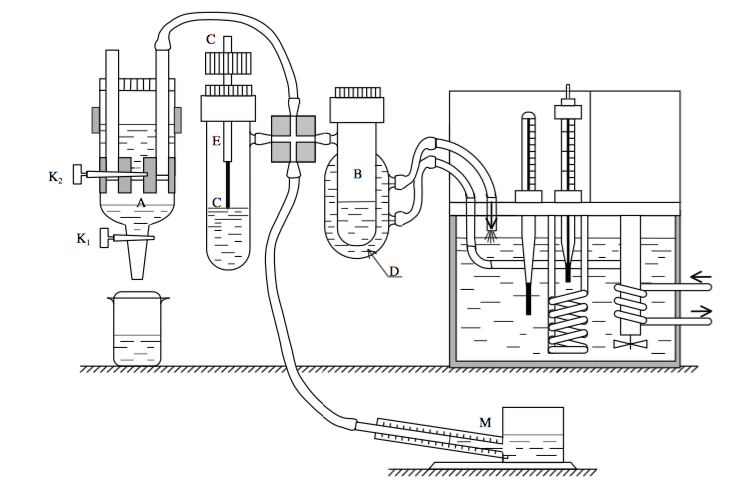
\includegraphics[width = 150mm]{station.png}
	\caption{Экспериментальная установка}
\end{figure}
Обычно кончик иглы лишь касается поверхности жидкости, чтобы исключить влияние гидростатического давления столба жидкости. Однако при измерении температурной зависимости коэффициента поверхностного натяжения возникает ряд сложностей. Во-первых, большая теплопроводность металлической трубки приводит к тому, что температура на конце трубки заметно ниже, чем в глубине жидкости. Во-вторых, тепловое расширение поднимает уровень жидкости при увеличении температуры. Это гидростатическое давление вычитается из падения лапласова давления вследствие уменьшения $\sigma$.\\
Обе погрешности можно устранить, погрузив кончик трубки до самого дна. Полное давление, измеренное при этом микроманометром, $P = \Delta P + \rho gh$. Заметим, что $\rho gh$ от температуры практически не зависит, так как подъем уровня жидкости компенсируется уменьшением ее плотности (произведение $\rho h$ определяется массой всей жидкости и поэтому постоянно). Величину $\rho gh$ следует измерить экспериментально двумя методами. Во-первых, замерить величину $P_1 = \Delta P' $, когда кончик трубки только касается поверхности жидкости. Затем при этой же температуре опустить иглу до дна и замерить $P_2 = \rho gh + \Delta P''$. Из-за несжимаемости жидкости можно положить $\Delta P' = \Delta P''$ и тогда $\rho gh = P_1 - P_2$. Во-вторых, при измерениях $P_1$ и $P_2$ замерить линейкой глубину погружения иглы $h_1$ и $h_2$.
\paragraph{Измерение радиуса иглы.} 
\begin{enumerate}
	\item Убедимся в исправности установки, для этого установим скорость падения капель примерно 1 капля в 5 секунд, добьёмся пробулькивания пузырьков (из-за несовершенства установки, пробулькивание будет 2-3 пузырька, что ухудшает экспериментальные данные).\\
	* --- \textit{игла находится в этаноле.}
	\item Максимальное давление при пробулькивании пузырьков и температуре $t_1 = 21 ^\circ C$ равно $ P_1 = 39$ дел.
	\item С помощью табличного значения коэффициента поверхностного натяжения этанола и формул (4), (5) вычислим $r$. Он получился равным $r = 0.1$ мм.\\
	* --- $\sigma_\text{этанола} = 22.8 \cdot 10^{-3}$ Дж/м$^2$ [Н.Б. Варгафтик. Справочник по теплофизическим свойствам газов и жидкостей, М., 1972 г. 2 изд. стр. 415 таблица 65] 
	\item Теперь с помощью микроскопа измерим диаметр иглы еще раз. Получили, что \\ $r = 0.4$~мм
	\item Различие в 3 мм можно объяснить тем, что при прямом измерении мы не учитываем толщину стенки иглы, а при косвенном измерении учитывается только ,,активный радиус,,. К тому же измерение давления имеет большую погрешность, причины этого описаны в п.1 этого раздела.
\end{enumerate} 
\paragraph{Поправка.} 
\begin{enumerate}
	\item Перенесем иглу в сосуд с водой.
	\item Максимальное давление при пробулькивании, когда игла находится на $h_1 = 5.5$ см, то есть лишь касается поверхности жидкости, равно $P_2 = 111$ дел.
	\item Утопим иглу до $h_2 = 6.3$ см. Максимальное давление при этом равно $P_3 =139$ дел.
	\item Тогда $\Delta P = 28$ дел --- поправка.
	\item Проверим, насколько точно мы измерили разность давлений. Рассчитав $\Delta h$ из известных $h_1$ и $h_2$ и из $\Delta P$.
	\begin{equation*}
	\Delta h = h_1 - h_2 = 0.8\,\text{см};\; \Delta h_\text{эксп.} = \dfrac{\Delta P}{\rho g} = 0.3\,\text{см}.
	\end{equation*}
	\item Значения не совпадают из тех же соображений, что и в п.1 предыдущего раздела.
\end{enumerate}
\paragraph{Обработка результатов.} \textit{Во время всех экспериментов множитель на манометре М был в значении 0.1}
\paragraph{Радиус иглы.} 
\begin{equation}
P_1 = 39 \cdot 0.1 \cdot 9.8 = 38.2\,\text{Па}
\end{equation}
Подставив табличное значения коэффициента поверхностного натяжения этанола $\sigma = 22.8\cdot 10^{-3}\,\text{Дж/м}^2$ в формулу (1), рассчитаем радиус иглы. 
\begin{equation}
P_1 = \dfrac{2 \sigma}{r}\then r = 0.1\,\text{мм}\\
\end{equation}
\paragraph{Зависимость $\sigma$ от $T$.} Снимем зависимость $\sigma(T)$ при нагревании воды и визуализируем их в виде таблицы.
\begin{table}[H]
	\centering
	\caption{Зависиомсть $\sigma$ от $T$}
	\begin{tabular}{cc|ccc|c}
		\toprule
		$T,\,^\circ C$ & $T,\,\text{К}$ & $P$, дел & $P - \Delta P$, дел & $P-\Delta P$, Па & $\sigma \cdot 10^3$, Н/м \\\midrule
		28            & 301            & 140.0      & 112.0                 & 109.76           & 54.88                    \\
		35            & 308            & 139.0      & 111.0                 & 108.78           & 54.39                    \\
		40            & 313            & 137.0      & 109.0                 & 106.82           & 53.41                    \\
		45            & 318            & 136.0      & 108.0                 & 105.84           & 52.92                    \\
		50            & 323            & 134.7   & 106.7              & 104.53         & 52.26                  \\
		55            & 328            & 132.5    & 104.5               & 102.41           & 51.21                   \\
		60            & 333            & 129.0      & 101.0                 & 98.98            & 49.49            \\ \bottomrule
	\end{tabular}
\end{table}
С помощью МНК рассчитаем $\frac{d\sigma}{dT}$.
\begin{equation}
\dfrac{d\sigma}{dT} = -0.16 \pm 0.01 \cdot 10^{-3}\,\frac{\text{Н}}{\text{м}\cdot\text{К}}
\end{equation} 
Теперь с помощью формул (2) и (3) рассчитаем $q$ и $U_\text{П}/F$ для каждой из температур и обобщим данные в таблице.
\begin{table}[H]
	\centering
	\caption{Итоговые данные}
	\begin{tabular}{c|ccc}
		\toprule
		$T$, К & $\sigma \cdot 10^{-3}$, Н/м & $q \cdot 10^{-3}$, Н/м & $\dfrac{U_\text{П}}{F} \cdot 10^{-3}$, Н/м \\\midrule
		301.0  & 54.88                       & 48.45                  & 103.33                                     \\
		308.0  & 54.39                       & 49.58                  & 103.97                                     \\
		313.0  & 53.41                       & 50.38                  & 103.79                                     \\
		318.0  & 52.92                       & 51.19                  & 104.11                                     \\
		323.0  & 52.26                       & 51.99                  & 104.26                                     \\
		328.0  & 51.21                       & 52.80                  & 104.00                                     \\
		333.0  & 49.49                       & 53.60                  & 103.09                                    \\ \bottomrule
		
	\end{tabular}
\end{table} 
\begin{figure}[H]
	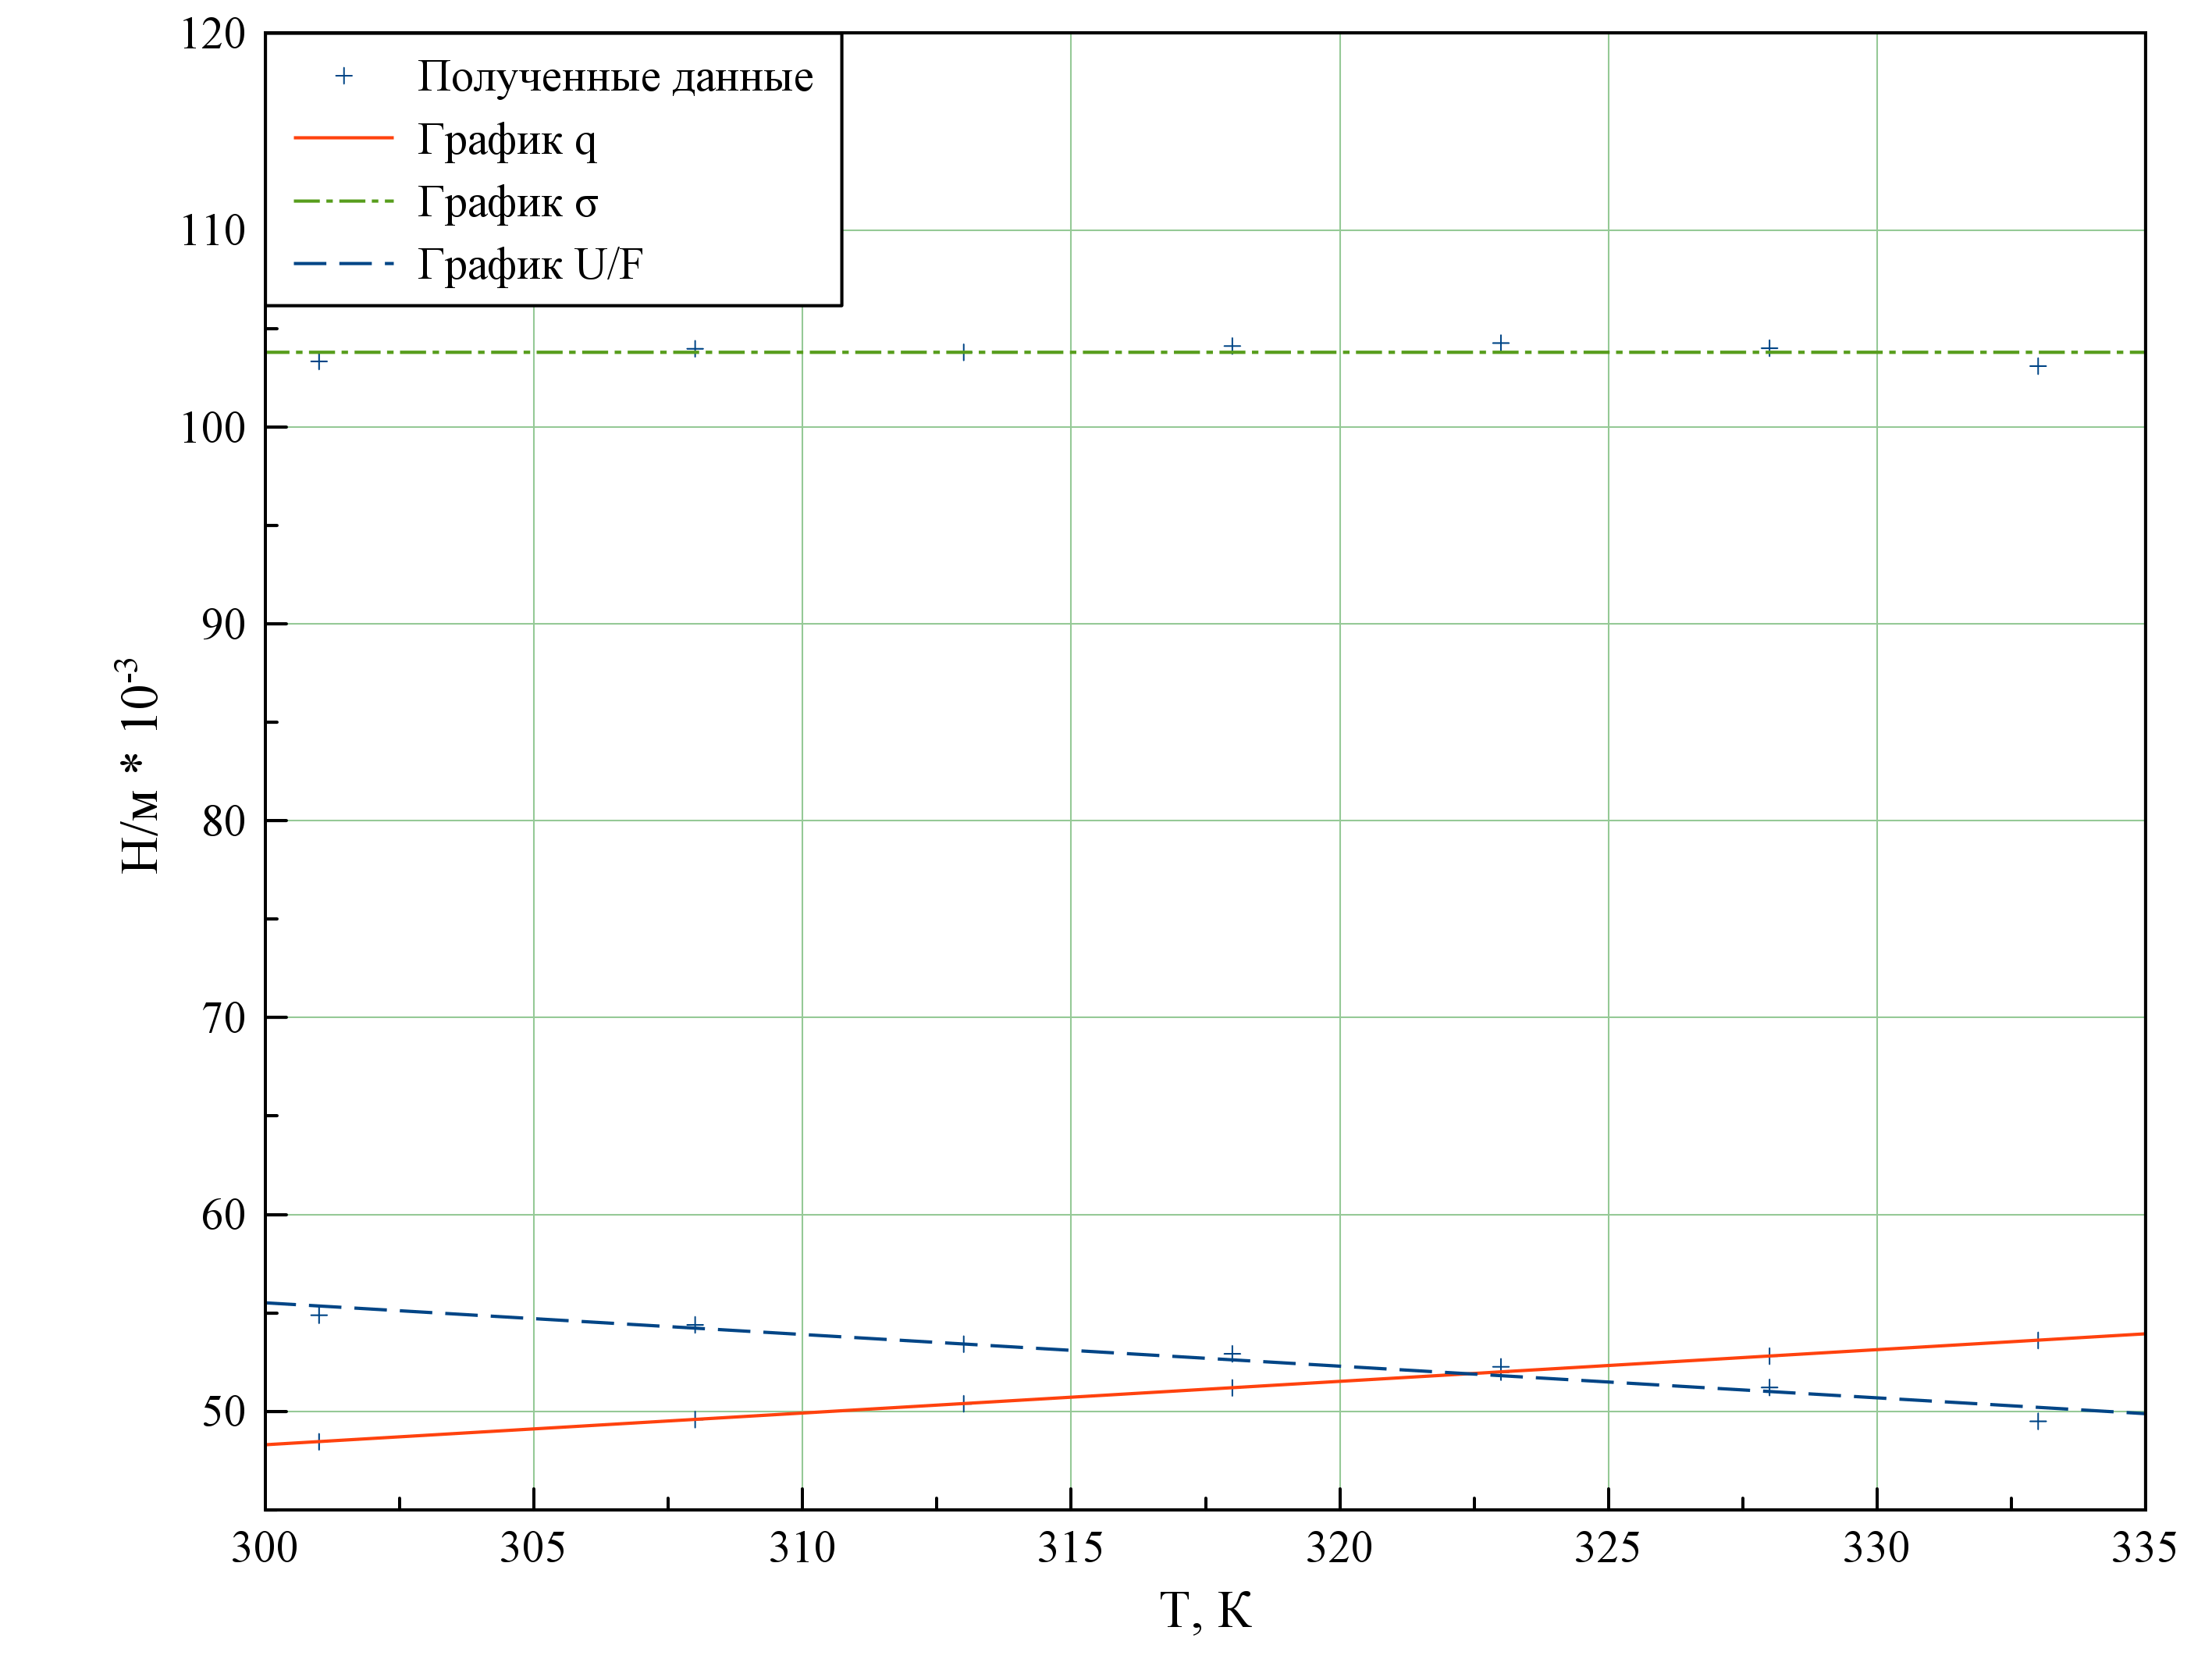
\includegraphics[width = 150mm]{Graph.png}
	\caption{Итоговые данные}
\end{figure}
\paragraph{Подведение итогов.}
Во время эксперимента были измерены коэффициенты поверхностного натяжения воды при разных температурах. Они оказалось недостаточно близки к табличным значениям [Таблица 11, Лаб. практикум]. Возможно, это обосновывается несовершенством экспериментальной установки, а именно плохим качеством иглы, из-за которого пробулькивание происходило по 2--4 пузыря воздуха.
\end{document}
